\documentclass[12pt]{article}

\usepackage{xcolor}
\usepackage{listings}
\usepackage{hyperref}
\usepackage{pdfpages}

\hypersetup{
    colorlinks=true,
    linkcolor=blue,
    filecolor=magenta,      
    urlcolor=cyan,
    pdftitle={HW05},
    pdfpagemode=FullScreen,
    }
\lstset{basicstyle=\ttfamily,
showstringspaces=false,
commentstyle=\color{red},
keywordstyle=\color{blue}
}

\renewcommand{\thesubsection}{\thesection.\alph{subsection}}

\title{Programming Assignment 5 \\ \small{ECE 759, Prof. TW Huang}}
\author{Sai Tadinada}
\date{}

\begin{document}
\maketitle

GitHub link to programming tasks: \\ \url{https://github.com/phantom3012/repo759/tree/main/HW05}

\section{Question 1}
\texttt{task1.cu} can be found at \url{https://github.com/phantom3012/repo759/blob/main/HW05/task1.cu}

\section{Question 2}
\texttt{task2.cu} can be found at \url{https://github.com/phantom3012/repo759/blob/main/HW05/task2.cu}
\section{Question 3}
\subsection{}
\texttt{vscale.cu} can be found at \url{https://github.com/phantom3012/repo759/blob/main/HW05/vscale.cu}
\subsection{}
\texttt{task3.cu} can be found at \url{https://github.com/phantom3012/repo759/blob/main/HW05/task3.cu}
\newpage
\subsection{}
\begin{figure}[ht]
    \centering
    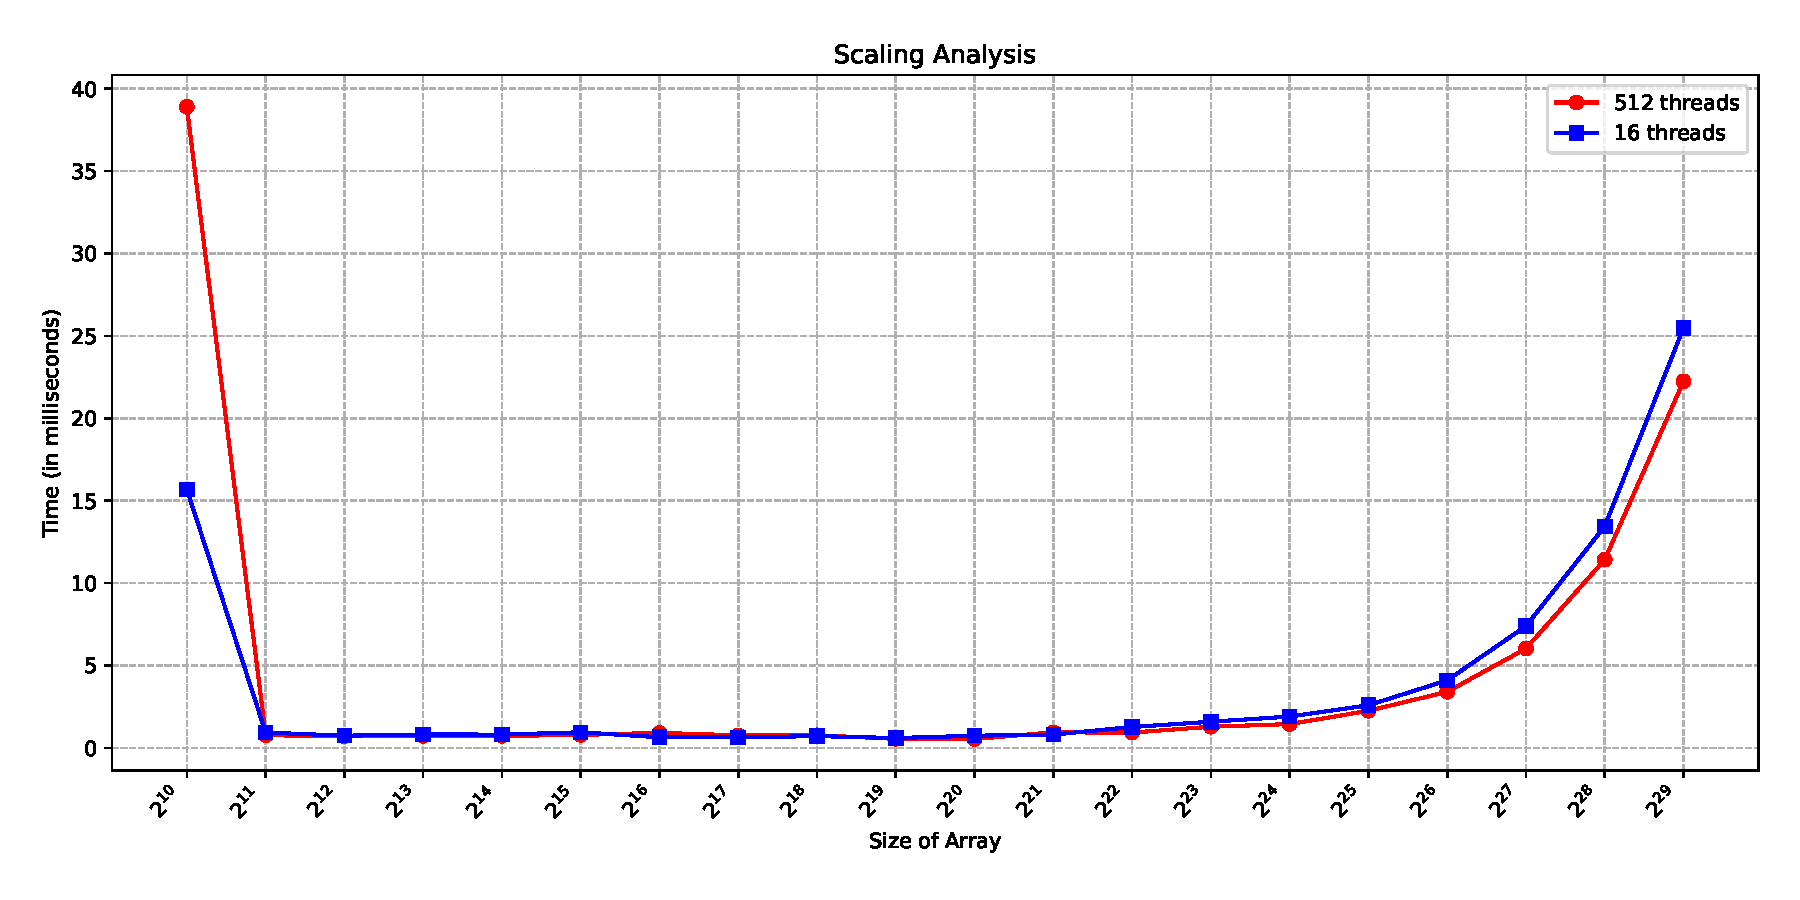
\includegraphics[width=\textwidth]{task3.pdf}
    \caption{Run time vs array size for different numbers of threads per block}
\end{figure}

\end{document}